% Korean draft based on PaperWorks/outlines/Outline_v16.3.md.
% Build: LuaLaTeX + BibTeX (see SETUP.md).
\documentclass[10pt,twocolumn,letterpaper]{article}
% Load ko.TeX before cvpr.sty under LuaLaTeX; the legacy luatexbase
% interface otherwise receives CVPR's active-percent definitions in Lua.
\usepackage{kotex}
\usepackage[review]{cvpr}
% Korean prose with the original CVPR page geometry and type size.
% TeX Gyre keeps the Times/Helvetica/Courier families available to LuaLaTeX.
\setmainfont{TeX Gyre Termes}
\setsansfont{TeX Gyre Heros}
\setmonofont{TeX Gyre Cursor}
\setmainhangulfont{Noto Serif CJK KR}[AutoFakeSlant=0.2]
\setsanshangulfont{Noto Sans CJK KR}
\setmonohangulfont{Noto Sans Mono CJK KR}
\usepackage{multirow}
\usepackage{array}
\usepackage{tabularx}
\usepackage{mathtools}
\usepackage{placeins}
\usepackage{tikz}
\usetikzlibrary{arrows.meta,positioning}
\newcommand{\method}{ScopeAD}
\newcommand{\AUPRO}{\ensuremath{\mathrm{AUPRO}_{0.05}}}
\newcommand{\pAUROC}{\ensuremath{\mathrm{pAUROC}_{0.05}}}
\newcommand{\missing}{\textemdash}
\newcommand{\red}[1]{{\color{red}#1}}
\newcommand{\todo}[1]{{\color{red}#1}}
\newcommand{\TODO}[1]{\textbf{\color{red}[TODO: #1]}}
\setlength{\emergencystretch}{1em}

\newcommand{\IAUROC}{\ensuremath{\mathrm{I\text{-}AUROC}}}
\newcommand{\PAUROC}{\ensuremath{\mathrm{P\text{-}AUROC}}}

\definecolor{cvprblue}{rgb}{0.21,0.49,0.74}
\usepackage[pagebackref,breaklinks,colorlinks,allcolors=cvprblue]{hyperref}
\def\paperID{*****}
\def\confName{CVPR}
\def\confYear{2026}
\title{ScopeAD: Observation Expansion and\\
Support-Referenced Asymmetric Fusion\\
for Few-Shot Industrial Anomaly Localization}
\author{Anonymous Authors}
\begin{document}
\maketitle
\begin{abstract}
소수의 정상 이미지만 사용하는 few-shot 산업 이상 국소화에서는 서포트에 없는 정상 외관 변화도 큰 최근접 거리를 만들 수 있어, 높은 점수만으로 정상 변동과 결함을 구분하기 어렵다.
본 논문은 제한된 서포트에서 비교 단서를 늘리기 위해 동결 백본의 표현 계층과 입력 해상도를 독립 매칭 단위로 확장하고, 그 거리를 정상 서포트 기준으로 통합하는 \textbf{\method}를 제안한다.
\method는 각 관측의 거리를 정상 참조 거리의 상위 분위수(Q95)로 나누어 단위를 맞추고, 깊은 계층의 평균에 얕은 계층을 작은 가중치로 더한다.
해상도 축에서는 위치별 점수 순위에 따라 Rényi 가중치를 적용하여 산술 평균에서 생기는 국소 반응의 희석을 줄인다.
백본의 추가 학습이나 쿼리 시점 파라미터 갱신은 사용하지 않는다.
MVTec AD 2에서 \method는 1--16-shot의 모든 조건에서 비교 방법보다 높은 \AUPRO, \pAUROC, \IAUROC를 기록했으며, 1-shot \AUPRO는 52.18\,\%로 차순위보다 5.87\,pp 높다.
구성 요소 분석에서는 다해상도 관측과 관측별 독립 매칭이 가장 큰 향상을 주었고, Q95 보정 아래에서 Rényi 집계가 추가 향상을 주었다.
MVTec AD와 VisA에서도 비교 방법과 대등한 성능을 보였다.
\end{abstract}

\section{서론}
\label{sec:intro}

% [문단 1: 문제 정의 — Few-shot 배경 및 High-Score Ambiguity 정의]
다품종 소량 생산과 잦은 라인 전환이 일어나는 제조 현장에서는 제품마다 결함 데이터를 충분히 모으거나 모델을 다시 학습하기 어려워, 소수의 정상 이미지만으로 결함 위치를 찾는 few-shot 이상 국소화가 실용적인 대안이 된다.
대표적인 방식은 동결된 사전학습 백본~\cite{dinov2}에서 추출한 정상 패치 특징으로 참조 뱅크를 만들고, 쿼리 패치와의 최근접 거리를 이상 점수로 쓰는 것이다~\cite{patchcore,anomalydino,superad}.
이 점수는 정상 쿼리 패치라면 참조 뱅크 안에 가까운 이웃이 있다는 가정에 기댄다.
그러나 실제 공정에서는 조명 드리프트, 부품 자세 변동, 표면 난반사 같은 획득 조건 변화가 계속 발생하며~\cite{aebad,mvtecad2}, 몇 장의 정상 서포트로는 이를 모두 담을 수 없다.
서포트에 없는 정상 변동이 나타나면 결함이 없는 패치도 최근접 거리가 커지고, 이 값은 실제 결함이 만든 큰 거리와 같은 구간에 놓일 수 있다.
따라서 큰 거리값만으로는 그 원인이 결함인지 서포트에 없던 정상 외관 변화인지 확정할 수 없으며, 본 논문은 이를 \textbf{High-Score Ambiguity}라 부른다(\cref{fig:intro-ambiguity}).
이 모호성은 오경보를 엄격히 제한하는 저-FPR 구간에서 특히 문제가 되는데, 정상 위치의 고점수로 인한 오경보를 줄이려고 판정 임계값을 높이면 함께 검출할 수 있는 결함 영역도 줄어들기 때문이다~\cite{aupimo}.

\begin{figure}[t]
\centering
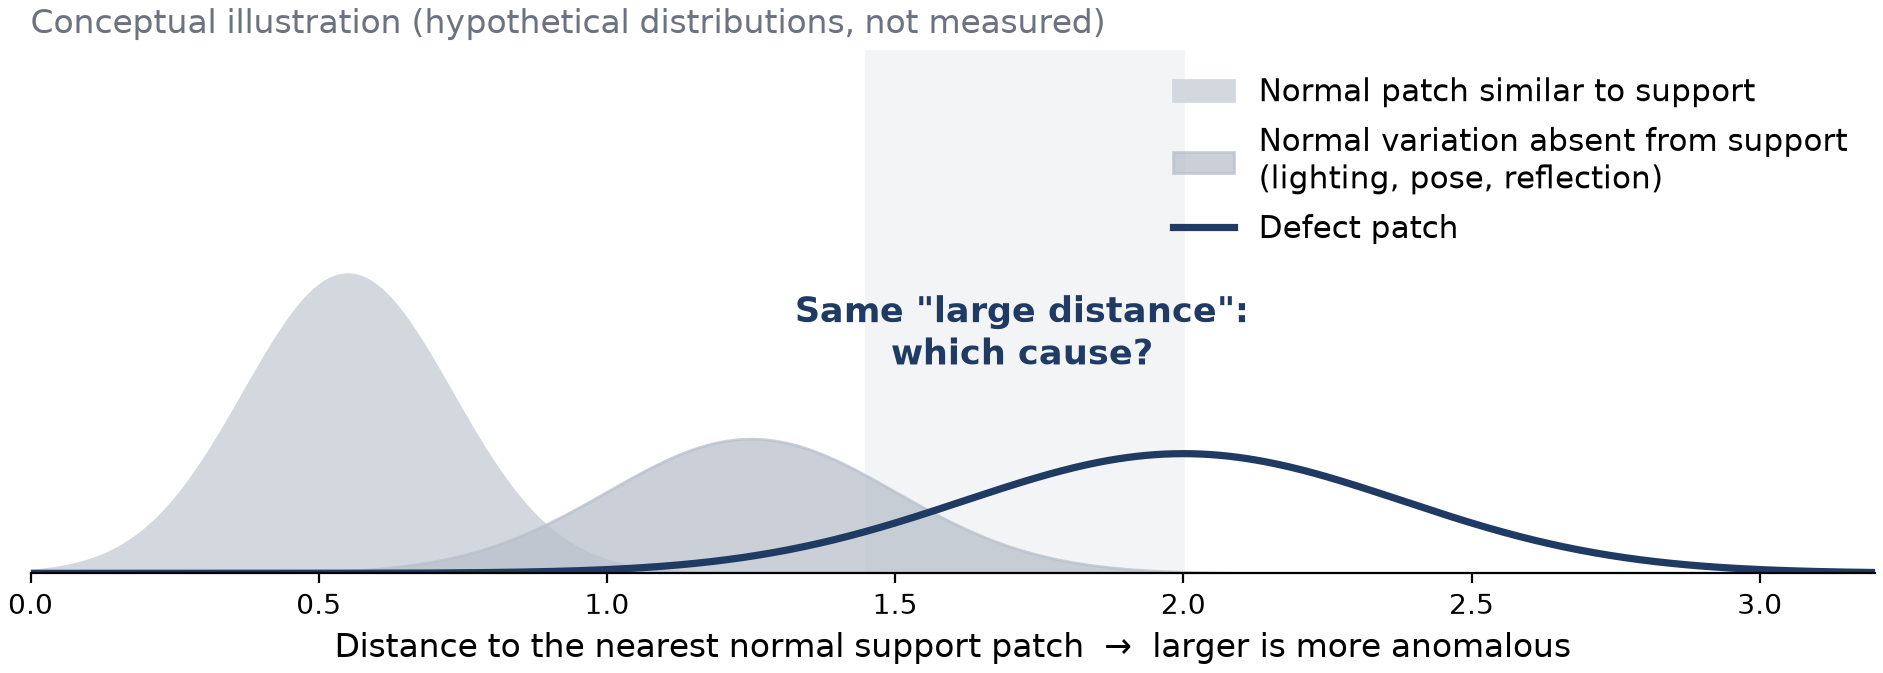
\includegraphics[width=\linewidth]{figures/fig_intro_ambiguity.png}
\caption{\textbf{Conceptual illustration of High-Score Ambiguity in few-shot inspection.} With sparse normal support, unobserved normal variations and true defects can both produce large nearest-neighbor distances. Raising the decision threshold to limit false alarms from normal high scores can also reduce defect coverage.}
\label{fig:intro-ambiguity}
\end{figure}

% [문단 2: 접근 방향 제안 — 계층·해상도 관측 확장 및 개별 매칭]
정상 서포트를 충분히 확보하면 더 다양한 정상 외관을 참조 뱅크에 담을 수 있지만, few-shot 조건에서는 사용할 수 있는 이미지 수가 제한된다.
따라서 한정된 서포트에서 결함 판단에 쓸 수 있는 시각적 단서를 충분히 확보하는 것이 중요하다.
본 논문은 이를 위해 표현 계층과 입력 해상도의 두 축으로 관측을 확장하되, 다층 특징을 단일 벡터로 묶어 하나의 이웃만 찾는 기존 접근~\cite{patchcore}과 달리 각 계층·해상도를 독립된 매칭 단위로 분리하는 방향을 취한다.
ViT는 계층마다 국소 외관과 전역 문맥을 반영하는 방식이 다르므로, 여러 계층의 특징은 서로 다른 수준의 비교 단서를 제공한다~\cite{raghu2021vision,ranftl2021vision}.
또한 입력 해상도는 각 패치가 나타내는 원본 영상의 공간 범위를 바꾸며, 패치 크기가 고정된 백본에서는 해상도가 높을수록 더 작은 영역이 하나의 토큰에 대응한다~\cite{shi2024scaling,fu2024featup}.
따라서 여러 계층과 해상도에서 참조 매칭을 개별적으로 수행하면, 미세한 국소 차이와 더 넓은 영역의 문맥적 차이를 각자의 표현·공간 척도에서 독립적인 비교 단서로 확보할 수 있다.

% [문단 3: 구체적인 문제 — 다관측 거리 통합 시의 척도 불균형과 오경보 유입]
그러나 이렇게 분리하여 확보한 다관측 매칭 거리를 하나의 이상 점수로 통합할 때, 원시 거리를 단순 합산하거나 평균하면 두 가지 구체적인 문제가 발생한다. 
첫째, 계층의 깊이와 입력 해상도에 따라 정상 참조 거리가 형성하는 기본 분포의 척도가 서로 다르므로, 보정 없이 동일한 계수를 적용하면 평소 거리 값이 큰 특정 관측이 최종 이상 점수를 일방적으로 지배하여 결합 결과가 왜곡된다. 
둘째, 관측 간 거리 척도를 맞추더라도 모든 계층을 동등한 비중으로 결합하면 계층별 민감도 차이로 인한 한계가 나타난다. 
얕은 계층의 특징은 미세한 국소 결함을 포착하는 데 유리하지만 조명이나 표면 질감 같은 정상 외관 변화에도 민감하게 반응하는 반면, 깊은 계층은 전역 문맥을 바탕으로 정상 변이에 비교적 강건하다. 
따라서 계층별 특성을 구분하지 않고 점수를 합치면, 얕은 계층에서 발생한 정상 변이의 큰 거리가 결합 점수에 그대로 유입되어 저-FPR 구간에서의 오경보(High-Score Ambiguity)를 다시 악화시킨다. 
결국 다관측 통합이 유효하려면 관측 간 거리 단위의 불균형과 계층별 오경보 민감도 차이를 동시에 해결해야 한다.

% [문단 4: 해결 방안 — ScopeAD (정상 참조 기반 선형 결합)]
이를 해결하기 위해 본 논문은 다관측 확장과 정상 참조 기반 선형 결합(Support-Referenced Linear Fusion)으로 구성된 \textbf{\method}를 제안한다. 
\method는 계층·해상도별 독립 뱅크에서 산출한 매칭 거리를 통합할 때, 단순 이상 맵 평균~\cite{superad}이나 단일 스케일 보정~\cite{freepatch}과 달리 관측별 정상 참조 척도와 계층별 고정 가중치를 함께 사용하여 선형 결합 계수를 정의한다. 
구체적으로 각 관측의 정상 서포트 내부 거리 분포로부터 기준 단위를 추정해 관측 간 척도를 정규화한 뒤, 깊은 계층의 정규화 점수 평균에 얕은 계층의 정규화 점수를 작은 고정 가중치로 더한다. 
이 선형 결합을 각 해상도에 적용한 후, 해상도별 맵을 원본 좌표에서 평균하여 최종 이상 맵을 생성한다. 
\method는 백본의 추가 학습이나 쿼리 시점 파라미터 갱신 없이 동작하며, 계층 가중치는 개발 평가에서 한 번 정한 뒤 모든 데이터셋과 shot 조건에 고정한다.

본 논문의 기여는 다음과 같다.
\begin{itemize}
  \item 제한된 정상 서포트에서 다양한 비교 단서를 활용하도록, 동결 백본의 계층·입력 해상도를 확장하고 관측별 매칭 거리를 독립적으로 유지하는 few-shot 이상 국소화 방법을 구성한다.
  \item 정상 서포트에서 추정한 기준 척도와 계층별 고정 가중치를 함께 사용하여 관측별 결합 계수를 정의하는 정상 참조 기반 선형 결합을 제안한다.
  \item 관측 구성과 결합 대안에 대한 비교로 전체 설계의 효과와 한계를 분석하고, MVTec AD 2~\cite{mvtecad2}의 다중 시드 저-FPR 성능, MVTec AD·VisA의 교차 데이터셋 성능 및 계산 비용을 보고한다.
\end{itemize}
\section{Related Work}
\label{sec:related}

\subsection{Frozen-Feature Reference Matching in Few-Shot AD}
\label{sec:related:matching}

소수의 정상 참조를 활용하는 이상 탐지 방법은 패치 매칭, 영상 정합, 특징 복원 및 정상 부분공간 모델링으로 나눌 수 있다.
패치 매칭 계열의 PatchCore~\cite{patchcore}는 사전학습 CNN의 다층 특징을 연결한 정상 메모리 뱅크와 최근접 거리를 사용하며, AnomalyDINO~\cite{anomalydino}와 SuperAD~\cite{superad}는 동결 DINOv2 특징을 활용한다.
RegAD~\cite{regad}와 FastRecon~\cite{fastrecon}는 각각 영상 정합과 특징 복원으로 정상 참조와의 차이를 측정하고, SubspaceAD~\cite{subspacead}는 정상 부분공간에 대한 잔차를 사용한다.
MVTec AD 2의 few-shot 연구~\cite{fewshotad2baseline}도 동결 특징의 계층 선택과 참조 수에 따른 결과를 분석한다.
이러한 정상 모델링 방식에 더해, ScopeAD는 최근접 매칭에서 계층·해상도별 관측을 확장하고 정상 참조 척도와 계층별 가중치를 함께 사용하는 점수 결합에 초점을 둔다.

\subsection{Multi-Scale Observation and Score Fusion}
\label{sec:related:fusion}

다층·다해상도 관측은 서로 다른 수준의 공간 정보를 결합하는 접근이다.
DPT~\cite{ranftl2021vision}는 여러 ViT 계층의 토큰을 학습된 디코더로 결합하고, S$^2$~\cite{shi2024scaling}는 동결 백본의 다중 척도 특징을 타일 처리와 재조립으로 구성한다.
이상 탐지에서는 PatchCore의 특징 연결과 SuperAD의 계층별 이상 맵 평균처럼 특징 또는 점수 단계에서 관측을 결합한다~\cite{patchcore,superad}.
FreePatch~\cite{freepatch}는 정상 참조 정보를 활용하여 패치 매칭 점수를 보정하는 접근이다.
이러한 접근은 관측을 특징 단계에서 합칠지 개별 매칭 후 점수 단계에서 합칠지, 그리고 정상 참조 정보를 결합에 어떻게 사용할지에 따라 구분할 수 있다.
ScopeAD는 계층·입력 해상도별 매칭 거리를 유지하고, 관측별 정상 참조 척도와 계층별 상대 가중치를 함께 사용하는 비대칭 결합으로 이를 통합한다.
구체적인 결합 계수와 정상 참조 추정은 \cref{sec:method:fusion}에서 정의한다.

\subsection{Distribution Shift and Low-FPR Localization}
\label{sec:related:shift}

획득 조건 변화에 대응하는 연구는 정상 외관의 변화와 결함을 구별하는 문제를 다룬다.
AeBAD 연구~\cite{aebad}는 실제 도메인 변화를 포함한 데이터셋과 masked multi-scale reconstruction 방법을 제안하며, MVTec AD 2~\cite{mvtecad2}는 조명 변화와 작은 결함을 포함한 평가 환경을 제공한다.
평가 측면에서 AUPIMO~\cite{aupimo}는 낮은 오경보 허용치에서의 국소화 품질을 측정하여 전체 곡선 지표를 보완한다.
ScopeAD는 정상 서포트로 정한 점수 척도와 고정 결합 규칙을 쿼리에 적용하며, 추가 학습이나 쿼리 적응 없이 분포 변화 조건의 저-FPR 국소화를 평가한다.
이때 정상 거리의 척도 보정과 고정 배포 임계값의 오경보율 보장은 구분한다.

\section{방법}
\label{sec:method}

\begin{figure*}[t]
\centering
\includegraphics[width=\textwidth]{figures/fig_scopead_overview.pdf}
\caption{\textbf{Overview of \method{}.} 
(a) 정상 서포트 표본으로부터 leave-source-out (1-shot의 경우 leave-token-out) 교차 매칭을 통해 48개의 독립 메모리 뱅크를 구축하고 참조 척도 $c_m$을 추정한다. 
(b) 코사인 1-NN 거리 $d_m$을 해당 척도로 정규화하여 공통 단위 점수 $z_m = d_m / c_m$을 도출한다. 
(c) 전역 문맥을 담은 깊은 계층을 주축으로 얕은 계층의 단서를 보조 결합하는 비대칭 선형 가중합을 수행한다. 
(d) 배그 평균 및 원본 해상도 보간 후, 각 픽셀 위치에서 정렬된 해상도 점수에 Rényi 순서 통계량 가중치를 적용하여 최종 이상 맵을 집계한다. 가중치는 해상도 크기가 아닌 점수 크기 순위에 따라 비대칭적으로 부여된다. 예시는 결함 픽셀 $p$의 실제 점수다(평균 1.41).}
\label{fig:method}
\end{figure*}

\method는 관측 확장(observation expansion)과 정상 참조 기반 점수 통합을 결합하여, 소수 서포트와 환경 변화로 인한 High-Score Ambiguity를 완화하는 이상 국소화 프레임워크다(\cref{fig:method}).
그 중심에서 \method는 표현 계층과 입력 해상도를 독립 매칭 단위로 분리하는 관측 확장을 수행하여, 특정 계층이나 해상도가 거리 계산을 지배하는 간섭을 배제하고 단일 영역에 대한 다각적 시각 단서를 확보한다.
이렇게 확보된 다관측 거리들을 효과적으로 결합하기 위해 세 가지 요소를 단계적으로 통합한다:
(1) 서포트 교차 매칭 분포의 상위 분위수로 기준 단위를 정렬하는 \textbf{정상 참조 척도화(Reference Scaling)},
(2) 전역 문맥을 담은 심층 특징을 기저로 삼고 얕은 계층의 반응을 수축 결합하는 \textbf{계층별 비대칭 결합(Asymmetric Layer Fusion)},
그리고 (3) 위치별 해상도 점수 순위에 따라 상위 반응을 안정적으로 보존하는 \textbf{Rényi 순서 통계량 집계(Rényi Order-Rank Aggregation)}이다.
추론 시 \method는 백본의 추가 학습이나 쿼리 적응 없이, 정상 서포트의 무감독 통계량만을 활용하여 단일 패스에서 픽셀 단위 결함 맵과 이미지 점수를 산출한다.

\subsection{문제 설정}
\label{sec:method:overview}

입력으로 $N$장의 정상 서포트 이미지 집합 $\mathcal{S} = \{x_1^s, \dots, x_N^s\}$, 테스트 쿼리 이미지 $x^q$, 그리고 동결된 사전학습 비전 트랜스포머(ViT) 백본이 주어진다.
특징을 추출할 백본 계층 집합을 $\mathcal{L}$, 입력 해상도(짧은 변 기준) 집합을 $\mathcal{R}$, 서브샘플 배그(bag) 수를 $B$로 정의한다.
본 연구에서는 $\mathcal{L}=\{5, 11, 23\}$, $\mathcal{R}=\{448, 672, 896, 1120\}$, $B=4$를 사용하여 총 $|\mathcal{L}| \times |\mathcal{R}| \times B = 48$개의 독립 관측을 구성한다(\cref{sec:experiments:setup}).
\method는 백본의 추가 학습이나 쿼리 적응(query adaptation) 없이, 오직 정상 서포트의 무감독 통계량만을 기반으로 픽셀 단위 결함 국소화 맵 $A(x^q) \in \mathbb{R}^{H \times W}$ 및 이미지 단위 이상 점수 $s(x^q) \in \mathbb{R}$를 산출한다.

\subsection{관측 확장과 독립 참조 매칭}
\label{sec:method:expansion}

\paragraph{관측별 독립 매칭 (Independent Matching).}
획득 조건이 달라지면 정상 영역이라도 특정 계층의 국소 질감이나 특정 해상도의 패치에서 거리가 급격히 상승할 수 있다.
기존처럼 다층 특징을 단일 벡터로 연결해 매칭하면~\cite{patchcore}, 분산이나 척도가 큰 특정 관측이 최근접 이웃 탐색 전체를 지배하여 정상 외관 변화에 따른 국소적 거리 상승이 다른 모든 계층의 비교 단서를 왜곡하게 된다.
이러한 간섭을 차단하기 위해 \method는 계층 $l \in \mathcal{L}$, 해상도 $r \in \mathcal{R}$, 배그 인덱스 $b \in \{1, \dots, B\}$의 조합 $m = (l, r, b)$를 개별 관측 단위로 분리하고, 각 관측마다 독립적인 정상 메모리 뱅크 $B_m$을 구축한다.
쿼리 이미지 $x^q$의 공간 위치 $p$에서 추출된 $\ell_2$ 정규화 패치 토큰 $f_m(x^q, p)$는 오직 대응하는 뱅크 $B_m$ 내에서만 독립적으로 최근접 이웃을 탐색하여 코사인 거리 점수를 계산한다:
\begin{equation}
  d_m(x^q, p) = \min_{u \in B_m} \left[ 1 - f_m(x^q, p)^\top u \right].
  \label{eq:cosine-dist}
\end{equation}
이 분리 매칭 구조에서는 각 관측이 고유한 표현·공간 척도 안에서 가장 가까운 정상을 개별적으로 찾는다.
그 결과 특정 척도에서 발생한 정상 외관 변동의 섭동이 다른 관측으로 전파되지 않고 격리되며, 국소 질감 단서와 전역 문맥 단서가 독립적인 거리 신호로 온전히 보존되어 후속 통합 단계에서 상호 검증의 기반을 마련한다.

\paragraph{패치 서브샘플 배깅 (Patch Subsample Bagging).}
입력 해상도가 증가함에 따라 서포트 패치 토큰의 수가 급격히 팽창하며, 단일 무작위 샘플링은 토큰 구성에 따른 추정 분산을 유발할 수 있다.
이를 완화하기 위해 각 해상도 $r$에서 서포트 이미지당 $K$개($K=256$)의 패치 토큰을 비복원 균등 추출하여 단일 배그를 구성하며, 서로 다른 난수 시드로 $B$개의 배그를 생성한다.
이때 일관된 공간 대응을 유지하기 위해 동일 배그 내의 모든 계층은 완전히 일치하는 공간 좌표의 토큰을 공유한다. 각 배그에서 산출된 이상 점수는 이후 \cref{eq:bag-mean}에서 앙상블 평균된다.

\subsection{정상 참조 기반 비대칭 선형 결합}
\label{sec:method:fusion}

독립적으로 획득한 원시 거리 $d_m$을 통합하기 위해서는 (1) 관측 간 척도 불균형(scale discrepancy)과 (2) 계층별 의미론적 민감도 차이를 단계적으로 다루어야 한다.
특징 공간의 차원과 표현 특성에 따라 원시 거리의 통계적 척도가 상이하므로(\cref{fig:scale-calib}), 보정 없이 결합하면 스케일이 큰 관측의 오경보가 결합 점수에 그대로 반영된다.
또한 척도를 정규화하더라도 국소 질감에 민감한 얕은 계층은 조명이나 자세 변화 등 정상 외관 변동에 큰 거리를 유발하기 쉽다.
따라서 \method는 서포트 교차 매칭 기반의 척도 $c_m$으로 단위를 정렬한 뒤, 비대칭 계층 가중치 $\alpha_l$을 적용하여 선형 결합을 수행한다.

\begin{figure}[t]
\centering
\includegraphics[width=\linewidth]{figures/fig_scopead_calibration_paper.pdf}
\caption{\textbf{정상 참조 보정(Q95)을 통한 관측 간 거리 척도 정렬.}
(a) Vial 2-shot 정상 쿼리에서 12개 관측(4개 해상도 $\times$ 3개 계층)의 상대 정상 척도. 보정 전(회색)에는 관측마다 정상 거리 척도가 최대 1.60배까지 불균일하여 특정 관측이 결합을 왜곡하지만, Q95 보정 후(청색)에는 모든 관측이 공통 기준선 근처로 균일하게 정렬된다(최대 편차 1.60배 $\rightarrow$ 1.24배).
(b) MVTec AD 2 전 클래스(8개 클래스 $\times$ 2개 shot)에서 관측 간 척도 불균형(최대/최소 척도 비율). 16개 조건 중 14개 조건에서 보정 후 척도 편차가 대각선($y=x$) 아래로 크게 감소하여 안정적으로 정렬됨을 보인다.}
\label{fig:scale-calib}
\end{figure}

\paragraph{서포트 교차 매칭 기반 척도 추정 (Cross-Validation Scale Estimation).}
미지의 쿼리 이미지와의 매칭 환경을 모사하기 위해, 서포트 집합 내부의 교차 매칭 거리 표본 $D_m$을 활용하여 관측별 기준 척도를 추정한다.
다중 샷($N > 1$) 환경에서는 동일 이미지 내의 자기 유사 패치와 매칭되어 거리가 과소 추정되는 편향을 방지하고자, 서포트 이미지 $i$의 토큰 부분집합 $B_m^{(i)}$를 해당 이미지를 제외한 나머지 뱅크 토큰들과 매칭하는 Leave-Source-Out (LSO) 방식을 적용한다:
\begin{equation}
  D_m^{\text{LSO}} = \bigcup_{i=1}^N \left\{ \min_{u \in B_m \setminus B_m^{(i)}} \left[ 1 - v^\top u \right] : v \in B_m^{(i)} \right\}.
  \label{eq:lso}
\end{equation}
단일 샷($N = 1$) 환경에서는 이미지 간 교차 비교가 불가능하므로, 단일 이미지 내에서 자기 자신을 제외한 타 위치 토큰들과 매칭하는 Leave-Token-Out (LTO) 표본을 대리 통계량으로 사용한다:
\begin{equation}
  D_m^{\text{LTO}} = \left\{ \min_{j \neq i} \left( 1 - v_i^\top v_j \right) : i = 1, \dots, K \right\}.
  \label{eq:lto}
\end{equation}

각 관측의 정상 거리 분포는 비대칭성과 꼬리 두께가 상이하므로, 특정 확률분포 형태를 가정하는 모수적 통계량 대신 비모수적 순서 통계량인 상위 분위수 $\mathcal{Q}_q$로 기준 척도 $c_m$을 정의하고 정규화 점수 $z_m$을 산출한다:
\begin{equation}
  c_m = \max \left\{ \mathcal{Q}_q(D_m), \, \epsilon \right\}, \qquad z_m(x^q, p) = \frac{d_m(x^q, p)}{c_m},
  \label{eq:scale-cm}
\end{equation}
여기서 $q=0.95$는 서포트 집합 내에서 관측되는 정상 거리의 상위 경계를 대표하는 분위수이며, $\epsilon=10^{-4}$는 수치적 안정성을 위한 하한값이다.
기준 척도 $c_m$은 각 관측 뱅크가 포착한 정상 외관 변동의 실질적 상한선을 뜻한다.
따라서 $z_m = d_m / c_m$ 변환은 이질적인 원시 거리들을 '정상 변동 상한 대비 초과율'이라는 동일한 무차원 판정선($z_m = 1.0$) 위에 정렬한다(\cref{fig:scale-calib}).
이를 통해 원시 거리의 절대적인 기저 크기가 큰 특정 계층이나 해상도가 결합 점수를 일방적으로 지배하여, 정상 외관 변동이 결합 점수에서 오경보로 전파되는 왜곡을 완화한다.

\paragraph{계층 간 비대칭 결합 (Asymmetric Layer Fusion).}
척도가 정렬된 점수 $z_m$ 공간에서도 계층 간 역할 차이가 존재한다.
조명이나 표면 텍스처 등 획득 조건이 달라지면 국소 외관에 반응하는 얕은 계층은 정상 영역에서도 거리가 크게 치솟기 쉽다.
반면 전역 문맥을 담은 심층 계층은 획득 환경이 변화하더라도 정상 구조의 의미론적 일관성을 유지하므로, 정상 영역의 점수를 상대적으로 낮게 보존하는 안정적인 기저 판정선을 제공한다.
이를 반영하여 깊은 계층들($\mathcal{L}_{\text{deep}}=\{11, 23\}$)의 정규화 점수 평균을 기저 점수로 삼고, 정상 변동에 취약한 얕은 계층($l=5$)은 작은 가중치 $\lambda=0.125$로 축소 결합한다:
\begin{equation}
  S_{r,b}(x^q, p) = \frac{1}{2} \sum_{l \in \{11, 23\}} z_{l,r,b}(x^q, p) + \lambda \, z_{5,r,b}(x^q, p).
  \label{eq:layer-fusion}
\end{equation}
이 비대칭 결합은 환경 변화로 인한 얕은 계층의 오경보 유입을 전역 문맥 기저선으로 억제하면서, 국소 미세 결함 단서만을 선별적으로 보완한다.
정규화 점수 정의($z_m = d_m/c_m$)에 따라, 이는 원시 거리 $d_{l,r,b}$를 계층 가중치 $\alpha = (0.125, 0.5, 0.5)$와 각 관측의 기준 척도 $c_{l,r,b}$의 비율인 $w_{l,r,b} = \alpha_l / c_{l,r,b}$로 선형 결합하는 것과 같다.

\subsection{다해상도 순서 통계량 집계}
\label{sec:method:aggregation}

앞선 계층 결합을 거친 이상 점수는 여전히 $R$개의 입력 해상도별 맵으로 분리되어 있다.
먼저 각 해상도 $r$에서 $B$개 배그의 점수를 평균하여 패치 서브샘플링에 따른 추정 분산을 완화한 뒤, 양선형 보간(bilinear interpolation)을 통해 모든 해상도 맵 $S_r$을 원본 이미지 크기 $(H, W)$로 공간 정렬한다:
\begin{equation}
  S_r(x^q, p) = \frac{1}{B} \sum_{b=1}^B S_{r,b}(x^q, p).
  \label{eq:bag-mean}
\end{equation}

\paragraph{Rényi 순서 통계량 집계 (Order-Statistics Aggregation).} 
공간 축이 정렬된 다해상도 점수 맵들을 결합할 때, 단순 산술 평균($1/R=0.25$)은 특정 해상도에서만 뚜렷하게 관측되는 유효 결함 피크를 타 해상도의 낮은 점수와 섞어 희석시킨다.
반대로 결함 피크를 보존하기 위해 단순히 최댓값($\max$)만을 취하면, 정상 영역에서 단일 해상도에 우연히 발생한 단발성 잡음 스파이크가 그대로 최종 결함 점수로 채택되어 오경보를 유발한다.
따라서 다해상도 결합에는 최상위 반응의 피크는 온전히 보존하면서도, 단일 관측 잡음의 돌출을 다관측 지지 반응으로 완충(damping)하는 비대칭 가중 체계가 필요하다.

이러한 상위 편향 가중치를 자의적인 휴리스틱 튜닝 없이 결정하기 위해, 이상 탐지의 극치 꼬리 거동(tail behavior)을 다루는 표준 지수 분포의 순서 통계량 기댓값 간격(Rényi representation, $a_k = \sum_{j=1}^k \frac{1}{R-j+1}$)을 참조 모형으로 채택한다.
조화 수열(harmonic sum)에 기반한 이 기댓값 구조는 최상위 순위로 갈수록 가중치가 자연스럽게 완만히 증가하는 특성을 갖는다.
$R=4$일 때 정규화된 Rényi 순위 가중치 $w = (\frac{1}{16}, \frac{7}{48}, \frac{13}{48}, \frac{25}{48}) \approx (0.063, 0.146, 0.271, 0.521)$를 통해 다해상도 결합 맵을 산출한다:
\begin{equation}
  \tilde{A}(x^q, p) = \sum_{k=1}^R w_k \, S_{(k)}(x^q, p).
  \label{eq:scale-renyi-mean}
\end{equation}
이 가중 체계는 다해상도 이상 맵 결합에 두 가지 실질적인 이점을 제공한다:
(1) 최상위 점수 순위에 약 52.1\%($25/48$)의 지배적인 가중치를 부여하여 특정 해상도에 집중된 결함 피크 신호의 희석을 직접적으로 방어한다.
(2) 동시에 차상위 순위들($k=2, 3$)에도 약 41.7\%($20/48$)의 완만한 지지 가중치를 분배함으로써, $\max$ 집계처럼 한 해상도에서만 외톨이로 튄 국소 잡음 스파이크가 최종 결함으로 과대 채택되는 불안정성을 효과적으로 완충한다.
특히 앞 절의 \textbf{정상 참조 척도 보정($c_m$)}이 모든 해상도의 정상 기저 점수를 $z=1.0$ 기준으로 균일화해 두었기 때문에, 특정 해상도의 기저 잡음이 상위 순위를 차지해 오경보를 유발하는 위험 없이 유효 결함 반응만을 안전하게 보존할 수 있다.
Rényi 집계와 보정의 상호작용 메커니즘 분석은 \cref{sec:experiments:mechanism}에서 다룬다.

\paragraph{이미지 수준 이상 점수.}
최종 픽셀 단위 결함 국소화 맵은 $A(x^q) = \tilde{A}(x^q)$로 정의된다.
이미지 수준 이상 점수 $s(x^q)$는 $A(x^q)$ 내 상위 1\% 픽셀 집합 $\Omega_{0.01}$($|\Omega_{0.01}| = \max\{1, \lfloor 0.01HW \rfloor\}$)의 평균값으로 정의된다:
\begin{equation}
  s(x^q) = \frac{1}{|\Omega_{0.01}|} \sum_{p \in \Omega_{0.01}} A(x^q, p).
  \label{eq:image-score}
\end{equation}

\section{실험 (Experiments)}
\label{sec:experiments}

본 절에서는 ScopeAD의 few-shot 성능을 비교하고, 관측 확장과 결합 설계가 결과에 미치는 영향을 분석한다. 주 비교에 이어 관측 구성과 계산 비용, 결합 대안, 획득 조건별 진단, 합성 열화 비교, 공식 private 평가 순으로 근거를 제시한다.

\subsection{평가 설정 (Evaluation Setup)}
\label{sec:experiments:setup}

\noindent\textbf{데이터셋 및 분할.}
MVTec AD 2~\cite{mvtecad2}는 실제 산업 환경의 조명 드리프트와 미세 결함을 포괄하는 8개 클래스 벤치마크다.
공개 개발 평가 세트인 \texttt{test\_public}은 총 1,084장(정상 379장, 결함 705장)으로 구성되며, 기준(Regular) 환경 외에 Shift 1--3 등의 획득 조건 변화를 포함한다.
정상 서포트 이미지는 \texttt{train/good}에서 고정 시드와 매니페스트로 선별한다.
교차 데이터셋 검증을 위해 기존 MVTec AD(15개 클래스)~\cite{mvtecad}와 VisA(12개 클래스)~\cite{visa} 벤치마크를 함께 평가한다.

\noindent\textbf{Few-shot 설정 및 비교군.}
클래스당 정상 서포트 이미지 수 $N$은 $\{1, 2, 4, 8, 16\}$으로 설정한다.
ScopeAD(Ours, linear0125)는 DINOv2 ViT-L/14 백본을 동결 사용하며, 계층 $\{5, 11, 23\}$과 4개 해상도 $\{448, 672, 896, 1120\}$, FP16 autocast, cap256, $z_d + 0.125\,z_5$ 결합을 적용한다.
비교 대상 방법군은 PatchCore~\cite{patchcore}, SuperAD~\cite{superad}, AnomalyDINO~\cite{anomalydino}, FastRecon~\cite{fastrecon}, RAD~\cite{rad}, SubspaceAD~\cite{subspacead}, RegAD~\cite{regad}다.
동일한 shot과 seed의 비교는 서포트 경로, 쿼리 및 평가기를 공유한다. 비교 파이프라인의 해상도 설정값은 1120을 기준으로 하며, ScopeAD는 짧은 변 길이의 최댓값을 1120으로 설정하고 종횡비를 유지한다. RegAD는 STN 제약으로 공식 224 설정을 유지한다. 이 비교는 백본, 전체 토큰 수 또는 계산량까지 일치시킨 비교는 아니다.
주요 평가 지표는 클래스 매크로 \AUPRO, \pAUROC, 그리고 이미지 단위 \IAUROC다.
각 클래스에서 AUPRO는 결함 연결영역별 검출 비율을 평균한 PRO 곡선을 FPR $[0,0.05]$에서 적분하고 0.05로 나눈다.
pAUROC는 같은 구간의 pixel ROC 면적에 무작위 기준 0.5, 완전 분류 기준 1의 표준화를 적용한다.
이미지 AUROC와 교차 데이터셋 표의 pixel AUROC는 전체 FPR 구간을 사용하며, 모든 지표는 클래스별 값을 동일 가중 평균한다.


\noindent\textbf{개발 조건과 실행 규약.}
결합 가중치는 AD2 \texttt{test\_public} 2-shot seed 0에서 선택했으므로, AD2 공개 결과는 개발에 사용된 벤치마크의 평가로 해석한다.
MVTec AD와 VisA에는 동일한 가중치를 적용한다. 각 평가 클래스의 뱅크 및 척도 추정에는 정상 서포트만 사용한다.
ScopeAD는 \cref{sec:method:aggregation}의 고점수 연결영역 후처리를 포함한다.
AD2 1/4/8-shot 반복 평가와 16-shot 용량 비교의 실행 기록에서, 잡음 진단에 따른 저해상도 전환은 모든 쿼리에서 비활성 상태였음을 확인했다.
따라서 이 실행에서는 각 구성에 지정된 해상도 집합을 모든 쿼리에 고정하여 사용했다.
% Provenance for refreshed metrics: results/remote_runs/dsba3/scopead_v18_q95_linear0125_fp16_20261012/combined/{strata_ad2,multiseed_ad2,capacity_cost_ad2}.
% Each refreshed macro was recomputed from eight class metrics.json files; noise_guard_summary.fired=0 was checked in every corresponding run_manifest.json.

\subsection{Few-shot 주 비교 (Few-shot Main Benchmark)}
\label{sec:experiments:main}

\begin{table*}[t]
\centering
\scriptsize
\setlength{\tabcolsep}{2.5pt}
\caption{MVTec AD 2 \texttt{test\_public} 해상도 설정값 1120 기준 few-shot 비교 (\%). 각 값은 3개 시드 평균 $\pm$ 표본 표준편차다. ScopeAD의 seed는 0, 1, 2이며 각 seed에서 8개 클래스를 평균한 뒤 시드 간 통계를 계산한다. $\dagger$ RegAD는 공식 체크포인트의 STN 제약으로 224 측정값을 병기했다. 굵은 글씨는 최고 평균값, 밑줄은 차순위다.}
\label{tab:mvtec_ad2_fewshot}
\begin{tabular}{r l r r r r r r r r}
\toprule
Shot & Metric & PatchCore & AnomalyDINO & FastRecon & RAD & SubspaceAD & SuperAD & RegAD (224)$^\dagger$ & Ours (ScopeAD) \\
\midrule
1 & AUPRO@0.05 & 38.45 $\pm$ 1.85 & 35.95 $\pm$ 2.24 & 14.92 $\pm$ 2.27 & 26.42 $\pm$ 1.71 & 44.87 $\pm$ 1.87 & \underline{46.31 $\pm$ 3.73} & 12.73 $\pm$ 0.38 & \textbf{51.31 $\pm$ 4.01} \\
   & pAUROC@0.05 & 64.19 $\pm$ 0.68 & \underline{70.67 $\pm$ 0.69} & 55.70 $\pm$ 0.67 & 59.57 $\pm$ 0.35 & 70.56 $\pm$ 0.56 & 70.13 $\pm$ 1.14 & 57.76 $\pm$ 0.30 & \textbf{72.93 $\pm$ 1.69} \\
   & I-AUROC & 65.51 $\pm$ 1.91 & 66.83 $\pm$ 1.08 & 58.10 $\pm$ 4.46 & 58.68 $\pm$ 3.03 & 67.02 $\pm$ 2.27 & \underline{67.68 $\pm$ 0.32} & 57.73 $\pm$ 1.82 & \textbf{73.47 $\pm$ 1.23} \\
\midrule
2 & AUPRO@0.05 & 42.25 $\pm$ 2.08 & 38.20 $\pm$ 1.90 & 16.73 $\pm$ 2.39 & 31.61 $\pm$ 1.47 & 45.90 $\pm$ 0.75 & \underline{49.80 $\pm$ 2.33} & 15.05 $\pm$ 0.30 & \textbf{56.03 $\pm$ 2.99} \\
   & pAUROC@0.05 & 65.43 $\pm$ 0.38 & \underline{72.26 $\pm$ 0.56} & 57.14 $\pm$ 1.03 & 61.78 $\pm$ 0.15 & 71.53 $\pm$ 0.18 & 71.52 $\pm$ 0.58 & 58.76 $\pm$ 0.49 & \textbf{75.86 $\pm$ 0.59} \\
   & I-AUROC & 67.53 $\pm$ 1.55 & 68.95 $\pm$ 3.84 & 57.63 $\pm$ 6.82 & 59.37 $\pm$ 2.54 & \underline{70.42 $\pm$ 1.79} & 70.19 $\pm$ 2.16 & 60.56 $\pm$ 3.94 & \textbf{74.93 $\pm$ 1.54} \\
\midrule
4 & AUPRO@0.05 & 46.94 $\pm$ 1.00 & 40.32 $\pm$ 0.75 & 21.88 $\pm$ 1.73 & 36.51 $\pm$ 1.02 & 47.14 $\pm$ 0.76 & \underline{54.25 $\pm$ 0.86} & 17.40 $\pm$ 1.07 & \textbf{58.73 $\pm$ 0.12} \\
   & pAUROC@0.05 & 66.90 $\pm$ 0.22 & 73.09 $\pm$ 0.91 & 59.26 $\pm$ 0.80 & 63.84 $\pm$ 0.41 & 72.45 $\pm$ 0.20 & \underline{73.59 $\pm$ 0.13} & 60.36 $\pm$ 0.48 & \textbf{76.94 $\pm$ 0.60} \\
   & I-AUROC & 68.62 $\pm$ 2.28 & 70.90 $\pm$ 0.97 & 59.73 $\pm$ 4.40 & 62.31 $\pm$ 4.84 & \underline{71.02 $\pm$ 0.56} & 70.97 $\pm$ 2.08 & 63.79 $\pm$ 2.34 & \textbf{75.88 $\pm$ 0.46} \\
\midrule
8 & AUPRO@0.05 & 49.98 $\pm$ 1.90 & 41.64 $\pm$ 1.01 & 27.32 $\pm$ 0.14 & 40.79 $\pm$ 0.79 & 47.28 $\pm$ 0.40 & \underline{55.44 $\pm$ 1.21} & 19.25 $\pm$ 0.64 & \textbf{59.74 $\pm$ 1.03} \\
   & pAUROC@0.05 & 68.22 $\pm$ 0.53 & 73.71 $\pm$ 0.20 & 61.74 $\pm$ 0.50 & 65.62 $\pm$ 0.69 & 72.56 $\pm$ 0.21 & \underline{74.31 $\pm$ 0.38} & 62.02 $\pm$ 0.32 & \textbf{77.51 $\pm$ 0.17} \\
   & I-AUROC & 69.20 $\pm$ 0.75 & \underline{71.29 $\pm$ 1.69} & 63.46 $\pm$ 4.29 & 65.84 $\pm$ 0.43 & 70.46 $\pm$ 1.18 & 70.75 $\pm$ 0.58 & 64.34 $\pm$ 1.05 & \textbf{75.99 $\pm$ 0.58} \\
\midrule
16 & AUPRO@0.05 & 52.73 $\pm$ 1.36 & 42.30 $\pm$ 1.25 & 35.23 $\pm$ 0.57 & 42.58 $\pm$ 1.10 & 47.63 $\pm$ 0.14 & \underline{55.89 $\pm$ 1.07} & 20.28 $\pm$ 0.80 & \textbf{60.06 $\pm$ 0.88} \\
   & pAUROC@0.05 & 69.36 $\pm$ 0.51 & 73.97 $\pm$ 0.23 & 65.63 $\pm$ 0.43 & 66.62 $\pm$ 0.89 & 72.78 $\pm$ 0.07 & \underline{74.60 $\pm$ 0.52} & 63.46 $\pm$ 0.76 & \textbf{77.61 $\pm$ 0.37} \\
   & I-AUROC & 69.00 $\pm$ 0.53 & \underline{72.07 $\pm$ 1.27} & 67.45 $\pm$ 1.16 & 67.60 $\pm$ 1.35 & 70.46 $\pm$ 1.07 & 69.79 $\pm$ 0.52 & 65.64 $\pm$ 1.34 & \textbf{75.92 $\pm$ 0.82} \\
\bottomrule
\end{tabular}
\end{table*}

표~\ref{tab:mvtec_ad2_fewshot}는 MVTec AD 2 \texttt{test\_public}에서의 few-shot 주 비교 결과다.
ScopeAD는 평가한 모든 shot에서 SuperAD보다 높은 평균 AUPRO를 보였다. 여기서 평균 차이는 관측된 효과이며, 통계적 유의성 검정의 결과는 아니다.
특히 16-shot에서 3-seed 평균 \textbf{60.06\,\% \AUPRO}를 달성하여 SuperAD(55.89\,\%) 대비 \textbf{+4.17\,pp}, pAUROC@0.05에서 \textbf{+3.01\,pp} 높은 성능을 기록했다.
1-shot AUPRO는 $51.31\pm4.01\,\%$로, seed 0의 $54.81\,\%$보다 평균이 낮고 서포트 선택에 따른 변동도 크다. 소수 참조에 대한 평균 성능과 표본 선택 민감도를 함께 고려해야 한다.

\begin{table*}[t]
\centering
\scriptsize
\setlength{\tabcolsep}{5pt}
\caption{MVTec AD 및 VisA few-shot 교차 데이터셋 비교 (Seed 0 단일 실행). 각 셀은 $\text{I-AUROC} \ / \ \text{P-AUROC}$ (전체 FPR 구간, \%) 순서다. 굵은 글씨는 최고값, 밑줄은 차순위다. ---는 해당 조건의 결과를 보고하지 않음을 뜻하며 순위에서 제외한다.}
\label{tab:mvtec_visa_fewshot}
\begin{tabular}{l r r r r r r r r r}
\toprule
Dataset & Shot & PatchCore & AnomalyDINO & FastRecon & RAD & SubspaceAD & SuperAD & RegAD & Ours (ScopeAD) \\
\midrule
MVTec AD & 1 & 88.12 / 96.22 & 92.52 / 94.49 & 88.84 / 96.60 & 80.83 / 93.25 & 89.25 / \underline{96.92} & \underline{92.54} / \textbf{96.93} & --- / --- & \textbf{92.76} / 96.77 \\
         & 2 & 92.67 / 96.97 & 95.17 / 95.56 & 93.51 / 97.29 & 84.15 / 94.27 & 90.95 / 97.24 & \underline{95.43} / \underline{97.36} & --- / --- & \textbf{96.13} / \textbf{97.39} \\
         & 4 & 95.06 / 97.37 & 95.92 / 96.07 & 95.61 / \textbf{97.87} & 85.38 / 94.67 & 91.35 / 97.16 & \underline{96.65} / \underline{97.70} & --- / --- & \textbf{96.99} / 97.68 \\
         & 8 & 96.13 / 97.80 & 96.67 / 96.45 & 96.76 / \textbf{98.16} & 87.85 / 95.29 & 92.94 / 97.17 & \underline{97.39} / \underline{97.95} & --- / --- & \textbf{97.60} / 97.93 \\
         & 16 & 98.15 / 97.99 & 97.48 / 96.80 & 98.52 / \textbf{98.38} & 90.29 / 95.61 & 92.51 / 97.19 & \textbf{98.94} / \underline{98.09} & --- / --- & \underline{98.74} / 98.05 \\
\midrule
VisA     & 1 & 86.09 / 95.56 & 87.06 / 95.62 & 84.65 / 96.75 & 72.67 / 95.37 & 85.44 / \textbf{98.09} & \textbf{90.29} / \underline{97.06} & 71.12 / 93.41 & \underline{89.88} / 96.73 \\
         & 2 & 87.87 / 96.29 & 90.64 / 96.63 & 87.67 / \underline{97.43} & 77.24 / 96.37 & --- / --- & \textbf{92.20} / \textbf{97.68} & 71.59 / 94.59 & \underline{92.15} / 97.32 \\
         & 4 & 89.52 / 96.92 & 91.37 / 97.57 & 89.21 / \underline{97.91} & --- / --- & --- / --- & \underline{92.94} / \textbf{98.02} & 76.42 / 96.14 & \textbf{94.19} / 97.82 \\
         & 8 & 92.36 / 97.18 & 93.11 / 97.99 & 91.53 / 98.11 & --- / --- & --- / --- & \underline{94.50} / \textbf{98.29} & 80.19 / 96.64 & \textbf{95.01} / \underline{98.25} \\
         & 16 & 93.64 / 97.30 & 93.53 / 98.30 & 93.38 / 98.32 & --- / --- & --- / --- & \underline{95.19} / \underline{98.43} & 81.22 / 96.98 & \textbf{95.99} / \textbf{98.49} \\
\bottomrule
\end{tabular}
\end{table*}

표~\ref{tab:mvtec_visa_fewshot}는 기존 MVTec AD 및 VisA 벤치마크에서의 교차 평가 결과다.
이미지 AUROC는 보고된 비교군 중 두 데이터셋의 모든 shot에서 최고 또는 차순위다.
반면 pixel AUROC는 MVTec AD 1/4/8/16-shot에서 3위이며 VisA 1-shot에서는 4위로, 지표별 우위가 일치하지 않는다.
표~\ref{tab:multiseed_visa_mvtec}는 2-shot과 16-shot의 세 서포트 선택에 따른 변동을 보여준다. 표의 0.00은 소수 둘째 자리까지 표시한 값이며 변동이 없음을 뜻하지 않는다.
이 비교는 전체 FPR 구간의 성능을 평가하므로 AD2의 low-FPR 결과와 구분한다.

\begin{table}[t]
\centering
\scriptsize
\setlength{\tabcolsep}{4pt}
\caption{ScopeAD 3-seed 교차 데이터셋 성능 (\%, mean $\pm$ sample SD).}
\label{tab:multiseed_visa_mvtec}
\begin{tabular}{l c c}
\toprule
Dataset & 2-shot (I-AUROC / P-AUROC) & 16-shot (I-AUROC / P-AUROC) \\
\midrule
MVTec AD & 96.04 $\pm$ 0.30 / 97.38 $\pm$ 0.04 & 98.52 $\pm$ 0.20 / 98.05 $\pm$ 0.00 \\
VisA     & 92.38 $\pm$ 1.04 / 97.40 $\pm$ 0.08 & 95.78 $\pm$ 0.18 / 98.50 $\pm$ 0.02 \\
\bottomrule
\end{tabular}
\end{table}

\subsection{관측 구성: 해상도와 매칭 방식}
\label{sec:experiments:observations}

\begin{table}[t]
\centering\scriptsize\setlength{\tabcolsep}{4pt}
\caption{단일 대 다중 해상도 비교 (linear0125, AD2, seed 0, \%).}
\label{tab:linear_res_ad2}
\begin{tabular}{l c c}
\toprule
해상도 구성 & 2-shot (AUPRO / pAUROC) & 16-shot (AUPRO / pAUROC) \\
\midrule
448 단독  & 51.14 / 75.80 & 52.01 / 76.52 \\
672 단독  & 54.38 / 74.97 & 55.01 / 76.17 \\
896 단독  & 52.65 / 73.46 & 55.12 / 74.62 \\
1120 단독 & 54.27 / 72.47 & 57.47 / 74.86 \\
\textbf{4개 해상도 결합} & \textbf{59.33 / 76.48} & \textbf{59.57 / 77.46} \\
\bottomrule
\end{tabular}
\end{table}

\noindent\textbf{동일 서포트의 다해상도 관측.}
표~\ref{tab:linear_res_ad2}에서 네 해상도 결합은 최선 단일 해상도보다 AUPRO가 2-shot에서 $+4.95$\,pp, 16-shot에서 $+2.10$\,pp 높다.
448 단독과의 16-shot 차이 $+7.56$\,pp는 고해상도 사용과 다해상도 결합을 함께 포함하므로, 다해상도 구성의 근거는 최선 단일 해상도와 용량 일치 대조군을 중심으로 해석한다.
이 비교는 정상 이미지 수를 늘리지 않고 입력의 공간적 관측 조건을 확장하는 선택을 지지한다. 추가 관측이 독립적인 정상 표본을 제공한다는 뜻은 아니다.

\noindent\textbf{특징 연결과 관측별 매칭.}
표~\ref{tab:component_ablation}의 layer concat 구성은 계층 특징을 연결한 뒤 하나의 최근접 이웃을 찾는다.
ScopeAD는 계층마다 이웃을 찾고 정상 참조 기반 비대칭 결합을 적용하며, 16-shot AUPRO가 concat보다 $2.09$\,pp 높다.
이 비교에서는 이웃 선택, 거리 기준화 및 계층 가중 방식이 함께 달라진다. 따라서 이는 전체 구성의 비교이며, bank 분리만의 독립 효과로 해석하지 않는다.

\subsection{용량 및 계산 비용}
\label{sec:experiments:cost}

\begin{table*}[t]
\centering\small\setlength{\tabcolsep}{5pt}
\caption{현재 선형 결합의 용량 및 비용 비교 (AD2 16-shot, seed 0, 8-class macro). 토큰 수는 이미지당·계층당·배그당 값이다. 지표는 AUPRO@0.05 / pAUROC@0.05 (\%). 비용은 클래스별 측정값의 평균이며, 시간은 피팅 초(s) 및 쿼리당 밀리초(ms), 메모리는 쿼리 단계 PyTorch peak allocated GiB다. 전체 GPU 메모리 사용량과는 다르다.}
\label{tab:resolution_control}
\begin{tabular}{l r c r r r}
\toprule
해상도 & 토큰 수 & AUPRO / pAUROC & Fit (s) & Query (ms) & Peak (GiB) \\
\midrule
4개 해상도 & 256 & 59.57 / 77.46 & 20.62 & 1526 & 3.07 \\
1120 단독 & 256 & 57.47 / 74.86 & 12.77 & 993 & 1.91 \\
1120 용량 일치 & 1024 & 57.14 / 75.49 & 14.42 & 1182 & 3.04 \\
4개 해상도 & 1024 & 59.17 / 77.56 & 27.04 & 1941 & 6.69 \\
\bottomrule
\end{tabular}
\end{table*}

표~\ref{tab:resolution_control}는 bank 용량과 실행 비용을 함께 비교한다.
4개 해상도에 각각 256개 토큰을 할당한 구성과 1120 단독에 1024개를 할당한 구성은 계층·배그당 총 bank 토큰 수가 같다.
다해상도 구성은 이 용량 일치 대조군보다 AUPRO가 $+2.44$\,pp 높지만, 쿼리 시간도 1182ms에서 1526ms로 증가한다.
따라서 bank 용량 통제와 계산량 통제를 구분해야 한다.
다해상도에서 토큰 수를 1024로 늘리면 AUPRO는 59.57에서 59.17로 감소하고 메모리 사용량은 증가하여, 더 큰 bank가 항상 유리하지는 않았다.

비용 측정은 FP16 autocast, batch size 1이며 CUDA 동기화를 포함한다.
각 클래스의 네 구성은 같은 GPU에서 측정했고 클래스별 측정값을 동일 가중 평균했다.
피팅 시간에는 서포트 디코딩, 특징 추출, bank 구축 및 척도 추정이 포함되며 모델 로딩, 서포트 선택 및 1회 warmup은 제외한다.
쿼리 시간에는 예측과 후처리가 포함된다. 이 값은 해당 실행 환경의 측정이며 비교 방법 전체의 속도 순위를 의미하지 않는다.

\subsection{정상 참조 기반 비대칭 결합의 대안 비교}
\label{sec:experiments:ablation}

\begin{table}[t]
\centering\scriptsize\setlength{\tabcolsep}{3pt}
\caption{결합 대안 및 관측 구성 비교 (AD2 \texttt{test\_public} 16-shot, seed 0, 8-class macro, \%). Full은 관측별 bank, q95, $\lambda=0.125$, 네 해상도를 사용한다. 결합 대안은 거리를 기준화하는 방식 또는 계층 가중치를 변경한다. 관측 구성 비교의 concat은 매칭과 결합을 함께 변경한다. $\Delta$는 Full 대비 AUPRO 차이(pp)이며 두 지표의 FPR 상한은 0.05다.}
\label{tab:component_ablation}
\begin{tabular}{l r r r}
\toprule
구성 & AUPRO & pAUROC & $\Delta$AUPRO \\
\midrule
\textbf{Full: q95, $\lambda=0.125$} & \textbf{59.57} & 77.46 & 0.00 \\
\multicolumn{4}{l}{\textit{결합 대안}} \\
정규화 제거 & 59.17 & \textbf{77.65} & $-0.40$ \\
계층 동일가중 ($\lambda=0.5$) & 58.21 & 76.31 & $-1.36$ \\
MAD 정규화 & 58.52 & 77.17 & $-1.05$ \\
\midrule
\multicolumn{4}{l}{\textit{관측 구성 비교}} \\
Layer concat bank & 57.48 & 74.80 & $-2.09$ \\
448 단일 해상도 & 52.01 & 76.52 & $-7.56$ \\
\bottomrule
\end{tabular}
\end{table}

식~\eqref{eq:linear-fusion}의 결합 계수 $w_{l,r,b}=\alpha_l/c_{l,r,b}$에 대해, 계층 가중치 $\alpha_l$과 정상 참조 척도 $c_{l,r,b}$를 각각 변경한 대안을 비교한다.
표~\ref{tab:component_ablation}은 대표 조건인 16-shot 결과를, 부록~\ref{sec:appendix:fusion}은 전체 가중치 및 shot별 정규화 결과를 제시한다.

\noindent\textbf{비대칭 가중과 동일가중.}
$\lambda=0.5$는 세 계층의 정규화 점수에 같은 계수를 부여하며, 전체 평균과 상수배 관계다.
$\lambda=0.125$는 이 동일가중 대안보다 AUPRO가 16-shot에서 $1.36$\,pp, 개발에 사용한 2-shot에서 $4.41$\,pp 높았다.
검사한 양의 가중치 중에서는 $0.125$가 두 shot에서 가장 높았으나, 16-shot에서 $0.25$와의 차이는 $0.09$\,pp로 작다(표~\ref{tab:lambda_sensitivity}).
이 결과는 깊은 계층에 더 큰 비중을 두는 결합을 지지한다. Deep-only인 $\lambda=0$ 비교가 없으므로 얕은 계층 추가 자체의 이득이나 정상 반응의 선택적 제거를 입증하지는 않는다.

\noindent\textbf{정상 참조 척도의 선택.}
q95는 MAD보다 모든 shot에서 AUPRO가 $0.76$--$1.69$\,pp 높았다(표~\ref{tab:norm_factorial_ad2}).
반면 미정규화 대비 AUPRO 차이는 1/2/4/8/16-shot 순서로 $-0.25$, $+0.27$, $-0.33$, $-0.01$, $+0.40$\,pp이며, pAUROC에서도 일관된 개선은 없다.
q95는 관측별 거리를 정상 참조 단위로 표현하여 비대칭 결합 계수를 정의하는 선택으로 사용한다. 이러한 구조적 역할과 식~\eqref{eq:scale-invariance}의 척도 불변성은 실제 성능 향상을 보장하지 않는다.

\subsection{획득 조건별 진단}
\label{sec:experiments:shift}

\begin{table}[t]
\centering\small
\caption{ScopeAD 선형 결합의 AD2 획득 조건별 성능 (16-shot, seed 0, \%). 네 조건이 모두 존재하는 동일한 7개 클래스(can, fabric, rice, sheet\_metal, vial, wallplugs, walnuts)의 macro이며 fruit\_jelly는 제외한다. 각 shift 번호는 데이터셋의 클래스별 획득 조건을 따른다.}
\label{tab:acquisition-strata}
\begin{tabular}{l r r}
\toprule
조건 & AUPRO@0.05 & pAUROC@0.05 \\
\midrule
Regular & 61.76 & 78.16 \\
Shift 1 & 60.48 & 78.10 \\
Shift 2 & 58.10 & 76.64 \\
Shift 3 & 59.45 & 77.04 \\
\bottomrule
\end{tabular}
\end{table}

표~\ref{tab:acquisition-strata}는 같은 클래스 집합에서 획득 조건별 성능을 분리한 진단이다.
Regular AUPRO 61.76에 비해 Shift 1--3은 58.10--60.48로 낮아, 고정 결합 이후에도 조건 변화에 따른 저하가 남는다.
이 결과는 공개 개발 세트 내부의 분석이며 미관측 환경에 대한 독립 검증이나 비교 방법 대비 shift 우위를 뜻하지 않는다.
% Legacy gated private results and fig_acquisition_shift_by_shot.pdf are excluded: they do not evaluate the current linear method.

\subsection{합성 열화 조건 비교}
\label{sec:experiments:corruption}

\begin{table*}[t]
\centering\scriptsize\setlength{\tabcolsep}{4pt}
\caption{MVTec AD 합성 열화 비교 (15개 클래스, 16-shot, seed 0, 열화 강도 3, 서포트는 열화 없음). 각 셀은 AUPRO@0.05 / pAUROC@0.05 (\%)이며, 굵은 글씨는 각 지표의 최고값, 밑줄은 차순위다. $\dagger$ FastRecon은 DINOv2-L/14 기반 국소 이웃 능형 복원 변형이며 원 논문의 재현 결과가 아니다. $\ddagger$ RegAD는 공식 구현과 구별되는 DINOv2 밀집 매칭 변형이다. RAD는 로컬 DINOv3 ViT-B/16 캐시 경로로 실행했다.}
\label{tab:corruption}
\begin{tabular}{l c c c c c}
\toprule
방법 & Clean & Brightness & Contrast & Defocus blur & Gaussian noise \\
\midrule
PatchCore & 83.97 / 88.80 & 83.43 / \underline{88.38} & 77.15 / 85.27 & 81.58 / 87.41 & \textbf{74.03 / 83.66} \\
AnomalyDINO & 77.62 / 85.31 & 72.54 / 82.61 & 72.08 / 82.48 & 70.69 / 81.06 & 33.02 / 66.81 \\
FastRecon$^\dagger$ & \textbf{85.74 / 90.82} & 77.53 / 86.35 & 69.72 / 84.47 & \textbf{82.35 / 88.90} & 57.70 / 77.37 \\
RAD & 80.12 / 87.03 & 78.70 / 86.04 & 74.96 / 84.33 & 70.44 / 81.13 & 49.23 / 72.05 \\
SubspaceAD & 83.89 / 86.98 & 80.45 / 84.91 & 78.49 / 83.39 & 78.17 / 83.39 & 64.61 / 78.01 \\
SuperAD & 84.49 / \underline{89.15} & \underline{83.68} / \textbf{88.47} & \underline{82.27} / \textbf{87.86} & \underline{82.17} / \underline{87.74} & \underline{71.10} / \underline{82.45} \\
RegAD$^\ddagger$ & 38.11 / 78.65 & 36.14 / 77.02 & 32.01 / 74.77 & 37.33 / 77.91 & 28.12 / 70.00 \\
\midrule
Ours (ScopeAD) & \underline{85.42} / 88.98 & \textbf{84.64} / 88.35 & \textbf{83.40} / \underline{87.59} & 81.46 / 86.38 & 68.43 / 80.19 \\
\bottomrule
\end{tabular}
\end{table*}

표~\ref{tab:corruption}은 Hendrycks와 Dietterich~\cite{hendrycks2019benchmarking}의 합성 열화 평가 방식을 따라 테스트 이미지에만 열화를 적용한 결과다.
ScopeAD의 AUPRO는 Brightness와 Contrast에서 비교군 중 가장 높고, Clean에서는 FastRecon 다음이다. 반면 Defocus blur에서는 FastRecon과 SuperAD보다, Gaussian noise에서는 PatchCore와 SuperAD보다 낮다.
Gaussian noise에서 ScopeAD의 AUPRO는 Clean 대비 16.99\,pp 낮아져, PatchCore의 9.94\,pp와 SuperAD의 13.39\,pp보다 하락 폭이 크다.
pAUROC에서는 어느 조건에서도 최고값이 아니며, Contrast에서만 차순위다.
따라서 이 결과는 ScopeAD가 합성 열화 전반에서 우위라는 근거가 아니라, 밝기·대비 변화에서의 강점과 잡음·초점 열화에서 남는 취약성을 함께 보여준다.
서포트에 열화를 적용하지 않은 단일 seed 평가이므로 조건 간 차이의 통계적 유의성은 검정하지 않았다. 비교군의 해상도와 백본 설정은 방법별로 다르다.

\subsection{공식 private 평가}
\label{sec:experiments:private}

\begin{table}[t]
\centering\scriptsize\setlength{\tabcolsep}{3pt}
\caption{MVTec AD 2 공식 private 평가 (8-class macro, \%). 각 셀은 \texttt{test\_private} / \texttt{test\_private,mix} 순서다. ScopeAD는 16-shot, seed 0 단일 제출이다. ClassF1과 SegF1의 임계값은 서포트를 제외한 \texttt{train/good}에서 정한다. SuperAD 행은 전체 학습 데이터 기준 게시값이며 few-shot 결과와 직접 순위화하지 않는다.}
\label{tab:private}
\begin{tabular}{l c c c}
\toprule
방법 & AUPRO@0.05 & ClassF1 & SegF1 \\
\midrule
ScopeAD (16-shot) & 65.21 / 63.25 & 76.57 / 77.68 & 37.71 / 34.00 \\
\midrule
SuperAD (전체 데이터)~\cite{superad} & 60.51 / 58.37 & 70.20 / 74.40 & 47.18 / 42.51 \\
\bottomrule
\end{tabular}
\end{table}

표~\ref{tab:private}은 공식 서버에 제출한 ScopeAD의 private 결과다(제출 상태 DONE, 2026-10-14 확인).
임계값은 서포트 제외 \texttt{train/good}의 8번째 간격 표본에서 클래스별 정상 픽셀 p95의 1.421배로 정했으며 private 레이블은 사용하지 않았다.
AUPRO는 두 조명 조건에서 게시된 전체 데이터 SuperAD보다 높지만, SegF1은 낮다. 두 방법은 정상 데이터 예산, 백본, 입력 크기, 후처리가 달라 직접 비교가 아니다.
이 결과는 단일 seed의 한 번 제출이며 같은 조건의 few-shot 비교군 private 결과는 없다.

\section{논의 및 한계}
\label{sec:discussion}

\noindent\textbf{관측 확장의 효과와 비용.}
다해상도 결합은 총 토큰 상한을 맞춘 단일 해상도 대조군보다 높은 \AUPRO를 보였고, 관측별 독립 매칭도 특징 연결보다 높은 성능을 보였다.
반면 여러 해상도를 추론하므로 단일 해상도보다 쿼리 시간과 메모리가 늘어난다.

\noindent\textbf{보정과 집계의 효과 범위.}
Q95 보정과 Rényi 집계의 결합 이득은 \AUPRO에서 나타났으며 \pAUROC로 이어지지 않았다.
클래스별로 효과의 방향이 다르고 fabric의 기여가 크므로, 이 이득을 모든 결함 유형에 대한 일관된 개선으로 볼 수는 없다.
또한 정상 영역의 추가 응답 감소는 점수 분포의 변화이며, 고정 임계값에서의 오경보율 감소를 직접 보여주지는 않는다.

\noindent\textbf{서포트 편차와 배포 임계값.}
관측 확장은 주어진 정상 표본의 비교 단서를 늘리지만 미관측 정상 외관을 직접 보지는 못하므로, 서포트 선택에 따른 성능 변동이 남는다(1-shot 표준편차 4.07\,pp).
또한 \AUPRO와 \pAUROC는 FPR 구간에 대한 적분 지표이므로, 실제 라인에 적용하려면 목표 오경보율에 맞춘 임계값 교정이 별도로 필요하다.

\section{결론}
\label{sec:conclusion}

본 논문은 동결 백본의 계층과 해상도를 독립 매칭 단위로 확장하고, 정상 참조 분위수 정규화, 비대칭 계층 결합, Rényi 순위 집계로 점수를 통합하는 \textbf{\method}를 제안했다.
MVTec AD 2의 few-shot 평가에서 \method는 모든 shot에서 비교 방법보다 높은 저-FPR 국소화 성능을 보였으며(16-shot \AUPRO{} 60.74\,\%), MVTec AD와 VisA에서도 경쟁력 있는 성능을 유지했다.

{\small
\bibliographystyle{ieeenat_fullname}
\bibliography{main}}
\clearpage
\appendix
\section{결합 규칙과 파라미터의 추가 분석}
\label{sec:appendix:fusion}

본문의 분석을 보완하기 위해 계층 가중치와 해상도 집계 대안, 보정과 집계의 메커니즘 분석을 제시한다.
계층 가중치와 집계 대안 표는 MVTec AD 2 \texttt{test\_public}, seed 0의 8개 클래스 macro이며, 메커니즘 분석은 별도로 명시한 3-seed 결과를 사용한다.

\subsection{계층 가중치}
최종 구성(Q95, Rényi)에서 $z_d=(z_{11}+z_{23})/2$에 더하는 얕은 계층 가중치 $\lambda$를 바꾸어 비교한다(\cref{tab:lambda_final}).
$\lambda=0.5$에서는 세 계층의 계수가 같다. $\lambda=0$은 얕은 계층의 점수 기여만 제외한다.

\begin{table}[!htbp]
\centering\small
\caption{얕은 계층 가중치 $\lambda$의 민감도 (MVTec AD 2, seed 0, Q95, Rényi, \AUPRO, \%). 굵은 값은 최고값이다.}
\label{tab:lambda_final}
\begin{tabular*}{\columnwidth}{@{\extracolsep{\fill}}lrr}
\toprule
$\lambda$ & 2-shot & 16-shot \\
\midrule
0 & 59.05 & 59.11 \\
0.0625 & 59.76 & 59.73 \\
0.125 (사용값) & \textbf{59.92} & 60.16 \\
0.25 & 59.32 & \textbf{60.36} \\
0.5 & 56.23 & 59.47 \\
\bottomrule
\end{tabular*}
\end{table}

얕은 계층을 제외하거나($\lambda=0$) 가중치를 0.5로 높이면 두 shot 모두 성능이 낮아진다. 16-shot에서는 0.25가 0.125보다 0.20\,pp 높아, 최적값은 shot에 따라 조금 다르다.

\subsection{해상도 집계 대안}
\label{sec:appendix:aggregation}
최종 구성의 특징, 뱅크, Q95 보정, 계층 가중치를 고정하고 해상도 집계 규칙만 바꾸었다(\cref{tab:aggregation_alternatives}).
선형 순위 가중치는 $(0.1, 0.2, 0.3, 0.4)$다.
두 순위 가중 집계는 Mean보다 \AUPRO가 높고, Rényi와 선형 가중의 차이는 0.1\,pp 이내다.
따라서 이 결과는 높은 순위에 큰 가중치를 주는 집계의 효과를 보여주며, 특정 Rényi 가중치가 다른 순위 가중치보다 뚜렷하게 낫다는 근거는 아니다.

\begin{table}[!htbp]
\centering\scriptsize\setlength{\tabcolsep}{3pt}
\caption{해상도 집계 대안 (MVTec AD 2, seed 0, Q95, \%). 각 셀은 \AUPRO{} / \pAUROC{}이며, 굵은 값은 열별 최고값이다.}
\label{tab:aggregation_alternatives}
\begin{tabular*}{\columnwidth}{@{\extracolsep{\fill}}lcc}
\toprule
집계 방식 & 2-shot & 16-shot \\
\midrule
Mean & 59.33 / \textbf{76.48} & 59.57 / 77.46 \\
Order (linear) & 59.91 / 76.45 & 60.08 / \textbf{77.55} \\
Order (Rényi, Ours) & \textbf{59.92} / 76.36 & \textbf{60.16} / 77.52 \\
\bottomrule
\end{tabular*}
\end{table}

\subsection{보정과 Rényi 집계의 메커니즘 분석}
\label{sec:appendix:mechanism}

\begin{figure*}[t]
\centering
\includegraphics[width=\textwidth]{figures/fig_scopead_calibration_mechanism.pdf}
\caption{\textbf{Q95 보정과 Rényi 집계의 결합 메커니즘 분석.}
MVTec AD 2, 2/16-shot, seed 0/1/2에서 같은 특징과 거리를 재사용했다.
(a) 상대 추가 응답 $E/\mu$의 Q95$-$None 변화. Normal은 정상 이미지, Background는 결함 이미지의 정상 배경, Defect는 결함 영역이다. 같은 픽셀 표본으로 조건 간 차이를 계산하고 이미지·seed·클래스 순으로 평균했다. 작은 점은 3-seed 평균 클래스 효과, 마름모와 오차 막대는 macro와 클래스 bootstrap 95\,\% 구간이다.
(b) None+Rényi 대비 순위만, 점수 크기만, 둘 다 보정한 경우의 \AUPRO{} 차이. 작은 점과 구간은 (a)와 같다.
(c) Q95 분모에 평균 1의 log-normal 오차를 넣었을 때 오차가 없는 경우 대비 \AUPRO{} 변화. 각 $\sigma$에서 seed별 3회 오차를 두 집계에 동일하게 주고 평균했다. 색은 shot, 점선/실선은 Mean/Rényi다.}
\label{fig:calibration-mechanism}
\end{figure*}

\noindent\textbf{상대 추가 응답($E/\mu$).}
Rényi 집계에서 정상 이미지의 $E/\mu$는 Q95 보정 후 2-shot에서 $7.74\!\rightarrow\!7.10$\,\%, 16-shot에서 $8.56\!\rightarrow\!7.55$\,\%로 감소했다(\cref{fig:calibration-mechanism}(a)).
결함 영역에서는 $5.34\!\rightarrow\!5.36$\,\%, $6.36\!\rightarrow\!6.11$\,\%로 변화가 작았다.
결함과 정상 배경의 $E/\mu$ 차이는 $+0.74/+0.80$\,pp 커졌고, 정상 이미지 $E/\mu$의 Q99는 $-1.30/-1.61$\,pp 줄었다.
이는 상대 추가 응답 분포의 변화이며, 고정 임계값에서의 오경보율 변화를 직접 측정한 것은 아니다.

\noindent\textbf{순위 변경과 점수 크기 변경의 분리.}
Q95로 순위만 정하고 원점수를 합산하는 조건과, 원점수 순위를 유지한 채 Q95 점수를 합산하는 조건을 비교했다(\cref{fig:calibration-mechanism}(b)).
순위만 바꾼 효과는 $+0.05/-0.14$\,pp인 반면, 크기만 바꾼 효과는 $+0.46/+0.70$\,pp로 최종 이득의 대부분을 차지했다.
따라서 보정의 효과는 주로 점수 크기의 조정에서 나온다.

\noindent\textbf{보정 오차에 대한 민감도.}
보정 분모에 평균 1의 log-normal 오차를 넣으면(\cref{fig:calibration-mechanism}(c)), $\sigma=0.3$에서 Mean의 \AUPRO 변화는 $-0.03/+0.06$\,pp인 반면 Rényi는 $-0.74/-0.47$\,pp였다.
Rényi 집계는 Mean보다 분모의 정확도에 더 민감하다.

\noindent\textbf{단위에 따른 분포 비교.}
$E/\mu$는 해당 픽셀의 평균 응답을 분모로 쓰므로 결함에서 $\mu$가 커지는 효과도 포함한다.
이를 확인하기 위해 다른 fold 정상 이미지 $\mu$의 Q95로 나눈 $E$도 측정했다.
이 값의 정상/결함 평균은 2-shot에서 $4.31\!\rightarrow\!3.80$ / $6.18\!\rightarrow\!6.19$\,\%, 16-shot에서 $4.57\!\rightarrow\!3.80$ / $8.01\!\rightarrow\!7.66$\,\%로, 정상 추가 응답이 줄고 결함 응답이 상대적으로 유지되는 방향은 같았다.
결함$-$배경 $E/\mu$ 차이 변화의 클래스 bootstrap 95\,\% 구간은 $[+0.06,+1.72]/[+0.00,+2.02]$\,pp이며, 16-shot 하한이 0에 가깝다.
정상 이미지 $E/\mu$의 Q99 변화 구간은 $[-2.29,-0.50]/[-3.00,-0.48]$\,pp이고, 감소한 클래스는 7/8과 6/8이다.

\begin{table*}[t]
\centering\small\setlength{\tabcolsep}{8pt}
\caption{\textbf{클래스별 검출 변화와 해상도 응답 집중도의 연관.} MVTec AD 2, 3-seed 평균. Coverage 상호작용은 $(\mathrm{Q95{+}R}-\mathrm{Q95{+}Mean})-(\mathrm{None{+}R}-\mathrm{None{+}Mean})$이며, GT 영역 coverage를 이미지 안에서 평균한 뒤 이미지와 seed를 평균한 값이다. 임계값은 정상 이미지의 교차검증으로 목표 FPR 1\,\%에 맞추었으며, 실제 평가 FPR은 조건마다 다르다. $\rho$는 Q95 상태의 응답 집중도와 Mean$\rightarrow$Rényi coverage 차이의 클래스 내 Spearman 상관이다.}
\label{tab:mechanism_class_effects}
\begin{tabular}{l r r r r}
\toprule
클래스 & 2-shot 상호작용 (pp) & 16-shot 상호작용 (pp) & 2-shot $\rho$ & 16-shot $\rho$ \\
\midrule
can & $-0.05$ & $-0.06$ & 0.48 & 0.39 \\
fabric & $+7.24$ & $+11.50$ & 0.56 & 0.31 \\
fruit\_jelly & $+0.23$ & $+0.72$ & 0.48 & 0.46 \\
rice & $-0.38$ & $-0.71$ & 0.38 & 0.22 \\
sheet\_metal & $-1.86$ & $-1.78$ & 0.48 & 0.43 \\
vial & $+0.12$ & $-0.18$ & 0.30 & 0.03 \\
wallplugs & $-0.19$ & $-0.59$ & 0.51 & 0.52 \\
walnuts & $+0.05$ & $+0.79$ & 0.29 & 0.30 \\
\midrule
Macro & $+0.65$ & $+1.21$ & --- & --- \\
fabric 제외 & $-0.30$ & $-0.26$ & --- & --- \\
\bottomrule
\end{tabular}
\end{table*}

\noindent\textbf{클래스와 이미지의 불확실성.}
\cref{tab:mechanism_class_effects}의 coverage 상호작용은 클래스에 따라 부호가 다르다.
클래스 bootstrap 구간은 0을 포함하지만, 서포트·임계값·클래스를 고정하고 이미지만 재표집한 구간은 $[+0.18,+1.16]/[+0.61,+1.92]$\,pp다.
두 구간은 서로 다른 변동을 나타내며, 후자는 클래스 구성이나 서포트 선택의 변동을 포함하지 않는다.

\noindent\textbf{결함 크기와 대비.}
GT 면적이 이미지의 0.1\,\% 미만인 작은 영역의 coverage 상호작용은 $+0.86/+1.53$\,pp지만 fabric을 제외하면 $-0.18/-0.06$\,pp다.
0.1--1\,\% 및 1\,\% 이상 구간은 can이 없어 7개 클래스 범위다.
회색조 대비(GT 영역 평균과 8픽셀 주변 정상 영역의 차이를 주변 표준편차로 나눈 값)와 결함 크기의 상관 방향은 클래스마다 달랐다.
따라서 작은 결함이나 저대비 결함 전반에서 이득이 있다고 보기는 어렵다.

\noindent\textbf{해상도 순위 점유율.}
\cref{fig:order-rank-diagnostic}는 seed 0에서 각 픽셀의 최고 점수를 낸 해상도의 비율이다.
Q95 보정 후 448의 정상 점유율은 47.5/50.7\,\%에서 33.9/36.4\,\%로 줄고, 16-shot 작은 결함의 1120 점유율은 14.5\,\%에서 29.2\,\%로 늘었다.
정상 픽셀의 1120 점유율도 13.7\,\%에서 22.3\,\%로 늘었으므로, 이 그림은 순위 편중의 변화를 보여주는 보조 자료로 사용한다.

\begin{figure}[tbp]
\centering
\includegraphics[width=\columnwidth]{figures/fig_scopead_order_rank_diagnostic.pdf}
\caption{\textbf{정상 참조 보정과 해상도 순위 점유율.} MVTec AD 2, seed 0, 8개 클래스 macro. 점선은 균등 점유율 25\,\%다.}
\label{fig:order-rank-diagnostic}
\end{figure}

\subsection{계층·해상도 보정 축의 분리}
\label{sec:appendix:calibration-axis}

\begin{table}[!htbp]
\centering\scriptsize\setlength{\tabcolsep}{3pt}
\caption{\textbf{Q95 보정 분모의 계층·해상도 성분 분리.} MVTec AD 2, 2/16-shot, seed 0/1/2 평균 \AUPRO{} (\%). Global은 배그별 공통 배율만, Layer/Resolution은 공통 배율에 해당 축 성분만, Separable은 두 축 성분을 함께 적용한다. Full은 원래 Q95다.}
\label{tab:calibration_axis}
\begin{tabular*}{\columnwidth}{@{\extracolsep{\fill}}lrrrr}
\toprule
& \multicolumn{2}{c}{2-shot} & \multicolumn{2}{c}{16-shot} \\
\cmidrule(lr){2-3}\cmidrule(lr){4-5}
분모 & Mean & Rényi & Mean & Rényi \\
\midrule
None & 56.12 & 56.32 & 59.73 & 59.72 \\
Global & 56.12 & 56.32 & 59.73 & 59.72 \\
Layer & 55.91 & 56.13 & 59.90 & 59.82 \\
Resolution & 56.26 & 56.87 & 59.89 & 60.55 \\
Separable & 56.02 & 56.78 & 60.02 & 60.73 \\
Full Q95 & 56.03 & 56.78 & 60.06 & 60.74 \\
\bottomrule
\end{tabular*}
\end{table}

\noindent\textbf{분모 분해.}
정상 서포트 Q95 $c_{l,r,b}$의 로그를 각 배그에서 다음과 같이 분해한다:
\begin{equation}
  \log c_{l,r,b}=\gamma_b+u_{l,b}+v_{r,b}+h_{l,r,b}.
  \label{eq:calibration-axis-factor}
\end{equation}
$\gamma_b$는 계층·해상도 전체 평균이고, $u_{l,b}$와 $v_{r,b}$는 각 축 평균에서 $\gamma_b$를 뺀 값이며, $h_{l,r,b}$는 잔여 항이다.
Global, Layer, Resolution, Separable은 각각 $\exp(\gamma_b)$, $\exp(\gamma_b+u_{l,b})$, $\exp(\gamma_b+v_{r,b})$, $\exp(\gamma_b+u_{l,b}+v_{r,b})$를 분모로 쓴다. Full은 원래 $c_{l,r,b}$이며 None은 1이다.
모든 축 개입은 배그 공통 척도를 유지하므로 Global을 대조로 사용한다.
특징, 뱅크, 계층 가중치, FP16을 고정하고 분모만 바꾸었으며(8개 클래스 $\times$ 2/16-shot $\times$ 3 seed), None과 Full의 결과는 \cref{tab:interaction_multiseed}와 일치한다.

\noindent\textbf{축 효과.}
Rényi 아래에서 Resolution$-$Global은 $+0.55/+0.82$\,pp이며, seed별 macro 효과는 2-shot $+0.56/+0.64/+0.45$\,pp, 16-shot $+0.82/+0.78/+0.87$\,pp로 모두 양수다.
Mean 아래의 같은 효과는 $+0.15/+0.15$\,pp로 작다.
Layer$-$Global은 Rényi 아래에서 $-0.19/+0.10$\,pp로 shot에 따라 방향이 달랐고, Full$-$Separable은 두 shot 모두 0.01\,pp 이내로 잔여 항의 macro 영향은 작았다.
다만 Resolution$-$Global에서 양의 효과를 보인 클래스는 두 shot 모두 8개 중 4개이고, fabric의 효과가 $+5.18/+7.26$\,pp로 크다.
클래스 bootstrap 95\,\% 구간은 $[-0.36,+1.99]/[-0.40,+2.80]$\,pp로 0을 포함하며, fabric을 제외하면 $-0.11/-0.10$\,pp다.

\subsection{평균 응답 조건부 분석과 영역·픽셀 가중}
\label{sec:appendix:conditional-mechanism}

\noindent\textbf{같은 평균 응답 구간에서의 비교.}
두 보정 조건의 같은 픽셀을 보정 전 평균 응답 $\mu$의 10분위 구간에 배정했다. 구간 경계는 다른 정상 fold에서 정했다.
이미지$\rightarrow$seed$\rightarrow$클래스 순으로 집계하면 정상과 배경의 Q95$-$None $E/\mu$ 변화는 두 shot 모두 10개 구간 전체에서 음수였다.
결함$-$배경 변화는 8개 클래스가 모두 관측된 구간(2-shot 5--9, 16-shot 6--9)에서 모두 양수였다.
따라서 평균 응답 수준이 다른 픽셀이 섞여서 생긴 현상으로 보기는 어렵다. 다만 보정 후의 $\mu$까지 고정한 비교는 아니다.

\noindent\textbf{Fabric의 영역 수와 결함 픽셀 수.}
Fabric의 GT 영역 192개 중 180개(93.75\,\%)는 이미지 면적의 0.1\,\% 미만이지만, 이 영역들은 전체 결함 픽셀의 1.39\,\%만 차지한다.
목표 FPR 1\,\% 임계값에서 Q95+Rényi$-$None+Rényi의 영역 평균 coverage 변화는 작은 영역에서 $+6.85/+10.41$\,pp, 나머지 영역에서 $-1.36/-0.84$\,pp다(2/16-shot).
같은 변화를 GT 픽셀 수로 가중하면 작은 영역의 TPR 기여는 $+0.06/+0.08$\,pp, 나머지는 $-2.66/-1.64$\,pp다.
즉 많은 작은 영역의 coverage 증가와 큰 영역의 손실이 함께 나타나며, 영역 단위 지표(\AUPRO)와 픽셀 단위 지표(\pAUROC)가 다르게 움직이는 이유를 설명한다.

\end{document}
